\documentclass[12pt]{article}

\usepackage[spanish]{babel}
\usepackage{hyperref}
\usepackage{graphicx}
\usepackage{listings}
\usepackage{color}
\usepackage{multicol}
\usepackage{amssymb}
\spanishdecimal{.}
\usepackage{enumitem}
\usepackage{here}
\usepackage{dsfont}
\usepackage{amsmath}


%% Título
\title{Matemáticas para las Ciencias Aplicadas I}
\title{
	Segunda Lista de Problemas \\
	\textbf{Primera Parte} \\
	\vspace{1ex}
	\large Matemáticas para las Ciencias Aplicadas I \\
	Facultad de Ciencias, UNAM}

%% Fecha
\date{\today}

%% Autor
\author{Flores Morán Julieta Melina \\ Zarco Romero José Antonio}

%% Se marca el inicio del documento.
\begin{document}

%% Comando para crear el título.
\maketitle

%1
\section{Ejercicio 3}
\begin{enumerate}[label=(\alph*)]
\item Aproximar el valor del límite
\[
\lim_{x \to 0}\frac{3^x-2^x}{x}
\]
hasta tres decimales mediante la construcción de una tabla de valores apropiada.

\item Confirme su aproximación utilizando evidencia gráfica.
\begin{figure}[h]
\centering
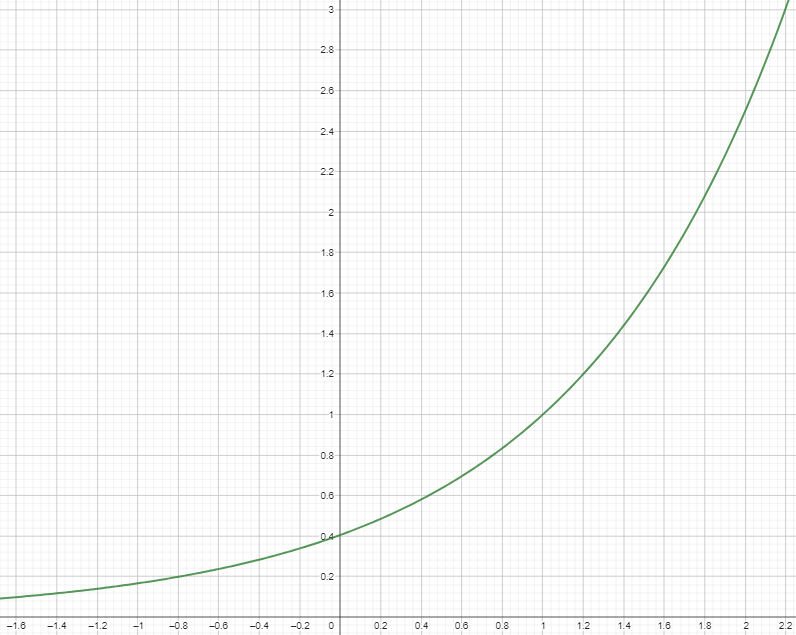
\includegraphics[width=1\textwidth]{../img/img_Lista2/ej3.png}
\end{figure}
\end{enumerate}

%2
\section{Ejercicio 9}
\[
\lim_{x \to +\infty}\frac{(2x-1)^5}{(3x^2+2x-7)(x^3-9x)}
\]

%3
\section{Ejercicio 18}
\[
\lim_{\theta \to 0^+} \ln (\sin 2\theta) - \ln (\tan \theta)
\]

%4
\section{Ejercicio 20}
\[
\lim_{x \to + \infty} (1+\frac{a}{x})^{bx} ~ ~ ~,~ ~ a,b>0
\]

%5
\section{Ejercicio 31}
Encuentre valores de $x$, si los hay, en los que la función dada no sea continua.
\begin{enumerate}[label=(\alph*)]
\item \[ f(x)=\frac{x}{x^2-1} \]
\item \[ f(x)= ~|~ x^3-2x^2 ~|~ \]
\item \[ f(x)=\frac{x+3}{~|~ x^2+3x ~|~} \]
\end{enumerate}

%6
\section{Ejercicio 36}
Supongamos que $f$ es continua en el intervalo $[0, 1]$, que $f(0) = 2$ y que $f$ no tiene ceros en el intervalo. Demuestre que $f(x) > 0$ para todo $x$ en $[0, 1]$.

\end{document}